%TODO: better pictures for bias etc instead of self-drawn, pictures in famous statistican potraits
\section{Descriptive Statistics}
%%%%%%%%%%%%%%%%%%%%%%%%%%%%%
	Descriptive statistics give us tools to summarize and interpret data.
	\begin{defi}[Statistics]{defi:stat}
		Analyzing characteristics of a sample to interpret characteristics of the population. 
	\end{defi}
	\begin{defi}[Probability Theory]{defi:prob}
		Knowing characteristics of a population to find the probability for a sample.
	\end{defi}		
	Why is it important to know your sample? Because knowing the variability in the dataset allows to find abnormalities. Such abnormalities can either be invalid data records which need to be filtered out, or remarkable observations pointing towards unexpected subpopulations, which deserve to learn more about them.
\subsection{Point Estimates}
	\subsubsection{Central tendency}
		\begin{defi}[Arithmetic Mean]{defi:mean}
			Consider a sample $x_1,x_2,...,x_n$ with the size $n$ from a population of the size $N$.
			\begin{align*}
				\text{Sample mean: }\;\bar{X}&=\frac{\sum\limits_{i=1}^{n}x_i}{n}\\
				\text{Population mean: }\;\mu&=\frac{\sum\limits_{i=1}^{N}x_i}{N}		
			\end{align*}			
		\end{defi}
		The \emph{arithmetic mean} is very common because it is easy to calculate, but sensitive to extreme values which can easily influence the value in their direction. A remedy to this problem is the usage of the \emph{median}.
		\begin{defi}[Median]{defi:median}
		In an ordered sample ($x_1\leq x_2 \leq ... x_n$), the median is $x_{int \frac{1}{2}}$ such that half of the observations are larger and the other half are smaller values. It is identical with the \nth{50}-percentile.
		\end{defi}
		Another useful measure is the \emph{mode}. If the distribution of a sample data is symmetric and unimodal (thus, has one mode), then there is a unique mode which is equal to the mean and equal to the median.
		\begin{defi}[Mode]{defi:mode}
			The mode is the value that occurs the most frequently.
		\end{defi}
	\subsubsection{Central relative standing}
		Consider an ordered sample $x_1\leq x_2 \leq ... x_n$. We can characterize the concept of the median to calculate percentiles. For example, the \nth{10}-percentile is such that 10\% of the observations are smaller and and 90\% are larger. The goal is to get information about the distribution of the data.
	\subsubsection{Measures of variability}
		Measures of variability quantify the dispersion of the data (typically around the mean).
		\begin{defi}[Range]{defi:range}
			The range is the difference between the highest and lowest value.
			\begin{equation*}
				x_{max}-x_{min}
			\end{equation*}
		\end{defi}
		\begin{defi}[Interquartile Range]{defi:iqrange}
			The interquartile range is the difference between the \nth{3} and the \nth{1} quartile.
			\begin{equation*}
			x_{75}-x_{25}
			\end{equation*}
		\end{defi}
		\begin{defi}[Variance]{defi:variance}
			The variance is the average sum of the squares of deviations to the mean.
			\begin{align*}
				\text{Sample variance: }\;s^2&=\frac{\sum\limits_{i=1}^{n}(x_i-\bar{X})^2}{n-1}\\
				\text{Population variance: }\;\sigma^2&=\frac{\sum\limits_{i=1}^{N}(x_i-\mu)^2}{N}
			\end{align*}
		\end{defi}
		Empirical experience has shown that dividing by $n-1$ gives better results for the variance with small sample sizes. The expressions $\bar{X}$ and $s^2$ are \emph{estimators} for the population mean $\mu$ and variance $\sigma^2$.
		\begin{defi}[Estimator]{defi:estimator}
			An estimator is a rule which tells how to combine and conclude
			sample data to obtain estimate a population characteristic.
		\end{defi}
		\begin{defi}[Standard Deviation]{defi:standarddev}
			The standard deviation is the square root of the variance.
			\begin{align*}
			\text{Sample standard deviation: }\;s&=\sqrt{s^2}\\
			\text{Population standard deviation: }\;\sigma&=\sqrt{\sigma^2}
			\end{align*}
		\end{defi}
		\begin{defi}[Empirical Rule]{defi:emprule}
			The empirical or 68–95–99.7 rule states the approximated percentage of values that lie within a certain range of the mean for data that is normal distributed.
			\begin{align*}
				\Pr(\mu-1\sigma \le X \le \mu+1\sigma) &\approx 0.6827 =68\% \\
				\Pr(\mu-2\sigma \le X \le \mu+2\sigma) &\approx 0.9545 =95\%\\
				\Pr(\mu-3\sigma \le X \le \mu+3\sigma) &\approx 0.9973 =99.7\%
			\end{align*}
		\end{defi}	
		\begin{defi}[z-score]{defi:z}
			A sample $x_1,x_2,...,x_n$ has the normalizing z-scores $z_1,z_2,...,z_n$.
			\begin{equation*}
				z_i=\frac{x_i-\bar{X}}{s}
			\end{equation*}
		\end{defi}
		\begin{exmp}[Expected Value of Random Variables]{exmp:expected}
			Consider a  sample $x_1,x_2,...,x_n$ as a random variable coming from $x\Rightarrow E(x) =\mu ,\, var(x) =\sigma^2$.\\
			Then $z$ is also a random variable: $z\equiv\frac{x-\mu}{\sigma}$.
			\begin{align*}
				E(z)&=E(\frac{x-\mu}{\sigma})=\frac{1}{\sigma}\left(E(x)-\mu\right)=0\\
				var(z)&=var(\frac{x-\mu}{\sigma})-\frac{1}{\sigma}var(x-\mu).
			\end{align*}
			For the random variable $y$: $var(y)=E\left((y-E(y)^2)\right)$.
			\begin{align*}
				var(y+\alpha)&=E\left((y+\alpha)-E(y+\alpha))^2\right)\\
				&=E\left((y-E(y))^2\right)\\
				&=var(y)
			\end{align*}			
		\end{exmp}
		\begin{defi}[Chebyshev's Theorem]{defi:chebyshev}
			For any sample, the proportion of observations whose z-score has an absolute value $z\leq k\,\epsilon\,\mathbb{N}^+$ is no less (so greater or equal) than $1-\frac{1}{k^2}$.
		\end{defi}
		\begin{align*}
			k=1\;\longrightarrow\; 1-\frac{1}{k^2}=1-\frac{1}{1^2}=0\;&\longrightarrow\;\text{no statement. Empirical rule: }68\%\\
			k=2\;\longrightarrow\; 1-\frac{1}{k^2}=1-\frac{1}{2^2}=\frac{3}{4}\;&\longrightarrow\;\geq 75\%\text{. Empirical rule: }95\%\\
			k=3\;\longrightarrow\; 1-\frac{1}{k^2}=1-\frac{1}{3^2}=\frac{8}{9}\;&\longrightarrow\;\geq 88.9\%\text{. Empirical rule: }99.7\%\\
		\end{align*}
		Named after the Russian mathematician Pafnuty Chebyshev, the theorem allows to make a statement about how much values are within an certain range. This information is less specific than that coming from the empirical rule, but Chebyshev's theorem is applicable to \emph{any} sample, regardless of its distribution whereas the 68–95–99.7 rule strictly requires normal distributed data.
	\subsubsection{Measures of the shape of a distribution}
		\begin{defi}[Skewness]{defi:skewness}
			The skewness is a measure for the degree of asymmetry of a distribution.
			\begin{align*}
				\text{Population skewness: }\;\gamma_1&={E}\left[\left(\frac{X-\mu}{\sigma}\right)^3 \right]= \frac{\mu_3}{\sigma^3}= \frac{E\left[(X-\mu)^3\right]}{( E\left[ (X-\mu)^2 \right] )^{3/2}}\\
				\text{Sample skewness estimator: }\; g_1&={E}=\frac{\frac{1}{n}\sum\limits_{i=1}^n (x_i-\bar{X})^3}{\left(\frac{1}{n}\sum\limits_{i=1}^n (x_i-\bar{X})^2\right)^\frac{3}{2}}
			\end{align*}			
			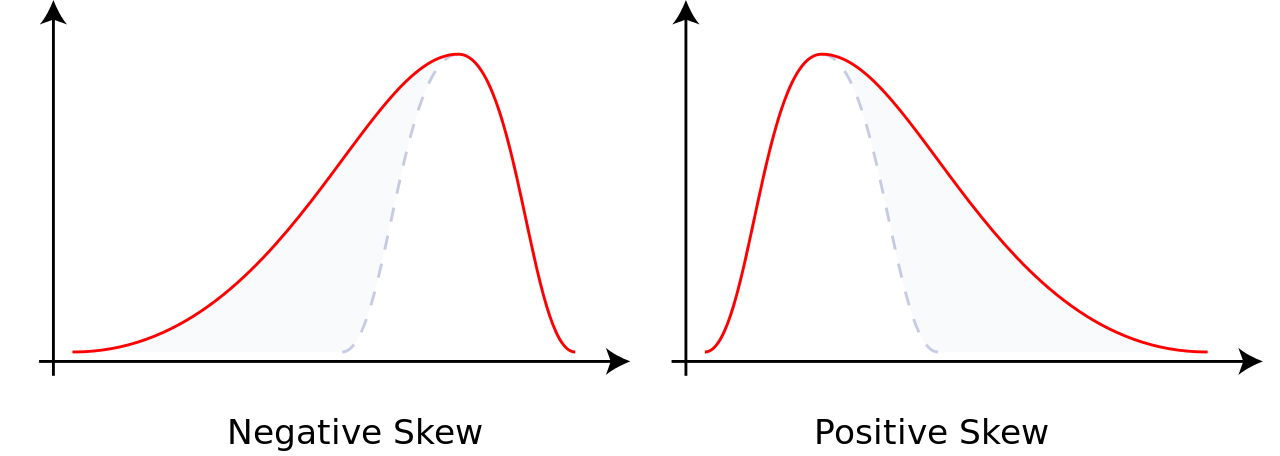
\includegraphics[width=\textwidth]{P01skew.png}	
			\credits{By Rodolfo Hermans (Godot) at Wikipedia Commons. CC BY-SA 3.0.}									
		\end{defi}
		For small sample sizes (but at least $x\geq 3$), the MATLAB-method delivers better estimates.
		\begin{equation*}
			G_1=\frac{\sqrt{n(n-1)}}{n-2}g_1
		\end{equation*}
		The skewness is the \nth{3} normalized moment when the distribution is seen as an area. The variance as shown in definition \ref{defi:variance} then is the \nth{2} central moment, whereas the mean shown in definition \ref{defi:mean} is the \nth{1} moment, i.e. the center of gravity.
		\begin{defi}[Kurtosis]{defi:kurt}
		The kurtosis (from the Greek word for \emph{curved}) is a measure about how heavy the tails of a distribution are compared to the center around the mean.
			\begin{align*}
			\text{Population kurtosis: }\;\kappa&=E\left(\left(\frac{x-\mu}{\sigma}\right)^4\right)\\
			\text{Sample kurtosis: }\; k_1&=\frac{\frac{1}{n}\sum\limits_{i=1}^n (x_i-\bar{x})^4}{\left(\frac{1}{n}\sum\limits_{i=1}^n (x_i-\bar{x})^2\right)^2}\\
			\text{Sample kurtosis estimator with bias correction: }\\
			k_0=\frac{n-1}{(n-2)(n-3)}\left((n-1)k_1-3(n-1)\right)&+3\\
			\text{The estimator requires: }\; n\geq 4,\qquad\lim\limits_{n\rightarrow\infty}\frac{(n-1)(n+1)}{(n-2)(n-3)}&=3
			\end{align*}					
			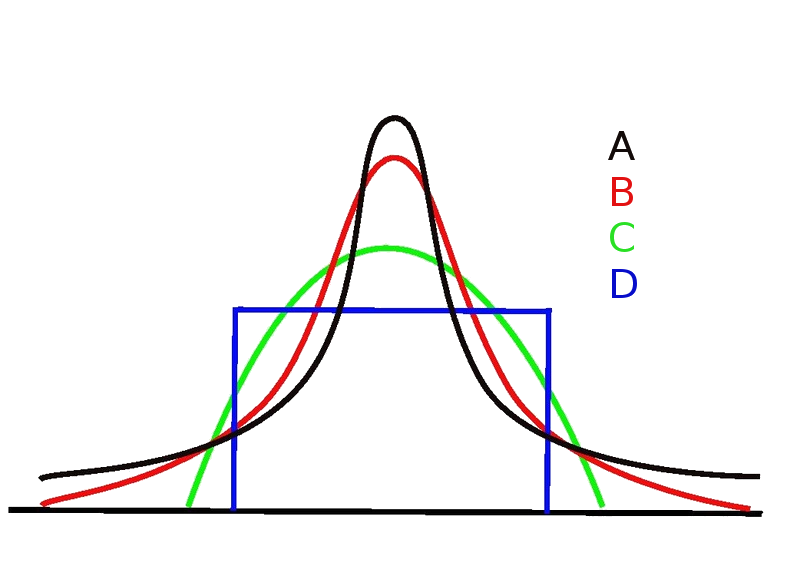
\includegraphics[width=\textwidth]{P00kurtosis.png}
			The graphic shows a normal distribution with different kurtosis, graph A has the highest.
			\credits{By Joxemai at Wikipedia Commons. CC BY-SA 3.0.}												
		\end{defi}
		The kurtosis gives us information on how prone to outliers a distribution is. Following the scheme of the skewness (\ref{defi:skewness}) as the \nth{3} moment, the kurtosis is the \nth{4} moment of a distribution. A normal distribution has  the kurtosis $\kappa=3$.
	\subsubsection{Measures of association}
		Often, we are interested in more than one variable in a time. The \emph{covariance} tells how two variables are related when one changes. The measure is not normalized and has an unit, so mostly informative is the sign. With a positive covariance, an increase in one value corresponds with a greater value for the other one, the covariance is positive. If the values change in different directions, the covariance is negative.
		\begin{defi}[Covariance]{defi:cov}
			Consider two random variables $x, y$.
			\begin{align*}
			\text{Sample covariance: }\;cov(x,y)_s&=\frac{\sum\limits_{i=1}^n(x_i-\bar{X})(y_i-\bar{y})}{n-1}\\
			\text{Population covariance: }\;cov(x,y)_p&=\frac{\sum\limits_{i=1}^N(x_i-\mu_x)(y_i-\mu_y)}{N}\\
			\mu_x&=E(x),\;\mu_y=E(y)
			\end{align*}					
		\end{defi}
		To address the problem that the covariance only indicated the direction in which to variables are related, it can be normalized to state the degree of linear association. This measure is called the \emph{correlation}.
		\begin{defi}[Correlation]{defi:cor}
			Consider two random variables $x, y$ with the covariance $cov(x,y)$. 
			\begin{align*}
			\text{Sample correlation: }\;r&=\frac{cov_{s}(x,y)}{s_x s_y}\\
			\text{Population correlation: }\;\rho&=\frac{cov_{p}(x,y)}{\sigma_x \sigma_y}\\
			|r|&\leq 1,\;|\rho|\leq 1
			\end{align*}
		\end{defi}		
		\begin{exmp}[Showing that the correlation is not greater than 1]{exmp:rho}
			Let $a_i=x_i-\bar{X}$ and $b_i=y_i-\bar{y}$. Let $f(z)=\sum (a_i z + b_i)^2 \geq 0$. Expand:
			\begin{align*}
				f(z)=z^2(a_1^2+a_2^2+\cdots+a_N^2)+z(2a_1 b_1+2a_2 b_2+\cdots+2a_N b_N)+(b_1^2+b_2^2+\cdots+b_N^2).
			\end{align*}
			Consider $f(z)=0$. There is no solution unless $a_i z + b_i = 0 \;\forall\; i, z$.		
			\begin{gather*}
				\alpha x^2+\beta x + \gamma = 0\\ \Delta=\beta^2-4\alpha\gamma\\
				\text{Cases }\;\begin{cases}
					\Delta>0, \qquad x^*=\frac{-\beta \pm \sqrt{\Delta}}{2\alpha}\\
					\Delta=0, \qquad x^*=\frac{-\beta}{2\alpha},\;\text{two equal square root solutions}\\
					\Delta>0, \qquad \text{no real solution}
				\end{cases}
			\end{gather*}	
			In this case,
			\begin{equation*}
				\Delta=4\left(\sum a_i b_i\right)^2-4\left(\sum a_i^2 \sum b_i^2\right)\leq 0.
			\end{equation*}
			This is necessarily since $f(z)\geq0$. Hence,
			\begin{align*}
				\left(\frac{\sum\limits_{i=1}^N(x_i-\mu_x)(y_i-\mu_y)}{N}\right)^2&\leq\frac{\sum\limits_{i=1}^N(x_i-\mu_x)^2}{N}\,\frac{\sum\limits_{i=1}^N(y_i-\mu_y)^2}{N}\\
				\left|\frac{\sum\limits_{i=1}^N(x_i-\mu_x)(y_i-\mu_y)}{N}\right|&\leq\sigma_x \sigma_y\\
				\left|\frac{\sum\limits_{i=1}^N(x_i-\mu_x)(y_i-\mu_y)}{N\sigma_x \sigma_y}\right|&\leq 1\\
				\Longrightarrow |\rho|&\leq 1
			\end{align*}
		\end{exmp}
\begin{famo}[John Graunt]{famo:graunt}
	\emph{John Graunt} (April 24, 1620 – April 18, 1674) was \emph{one of the first demographers}, though by profession he was a haberdasher (i.e., he sold small articles for sewing, such as buttons, ribbons, zips).
	
	He was born in London, the eldest of seven or eight children of Henry and Mary Graunt. His father was a draper who had moved to London from Hampshire. In February 1641, John Graunt married Mary Scott, with whom he had one son and three daughters.
	
	He worked in his father's shop until his father died in 1662, and became influential in the City. He served in various ward offices, becoming a common councilman about 1669–71, warden of the Drapers' Company in 1671 and a major in the trained band.
	
	His house was destroyed in the Great Fire of London and he encountered other financial problems leading eventually to bankruptcy. His daughter became a nun in a Belgian convent and Graunt decided to convert to Catholicism at a time when Catholics and Protestants were struggling for control of England and Europe, leading to prosecutions for recusancy. He died of jaundice and liver disease at the age of 53.
	
	With William Petty, \emph{he developed early human statistical and census methods that later provided a framework for modern demography}. He is credited with producing the first life table, giving probabilities of survival to each age. In addition, he is considered one of the first experts in epidemiology, since his famous book was concerned mostly with public health statistics.
	
	His book \enquote{Natural and Political Observations Made upon the Bills of Mortality} (1663) used analysis of the mortality rolls in early modern London as Charles II and other officials attempted to create a system to warn of the onset and spread of bubonic plague in the city. Though his system was not fully created, Graunt's work resulted in the first statistically based estimation of the population of London.
	
	He presented his work to the Royal Society and was subsequently elected a fellow in 1662 with the endorsement of the King. 
	\credits{Source: \url{https://en.wikipedia.org/wiki/John_Graunt}}
\end{famo}\pagebreak
\subsection{Methods for Displaying Data}
	Visualizing the data is useful for
	\begin{itemize}
		\item detecting influential observations,
		\item identifying outliers, and
		\item inspecting data and understanding its distributions. 
	\end{itemize}
	\subsubsection{Histograms}
		Histograms as in figure \ref{fig:hist} are used to display the frequency or density of different values. The values are classified in \emph{bins} representing a range of values the variable of interest can take.			
		\begin{fig}[Histogram]{fig:hist}{!htb}
			\centering
			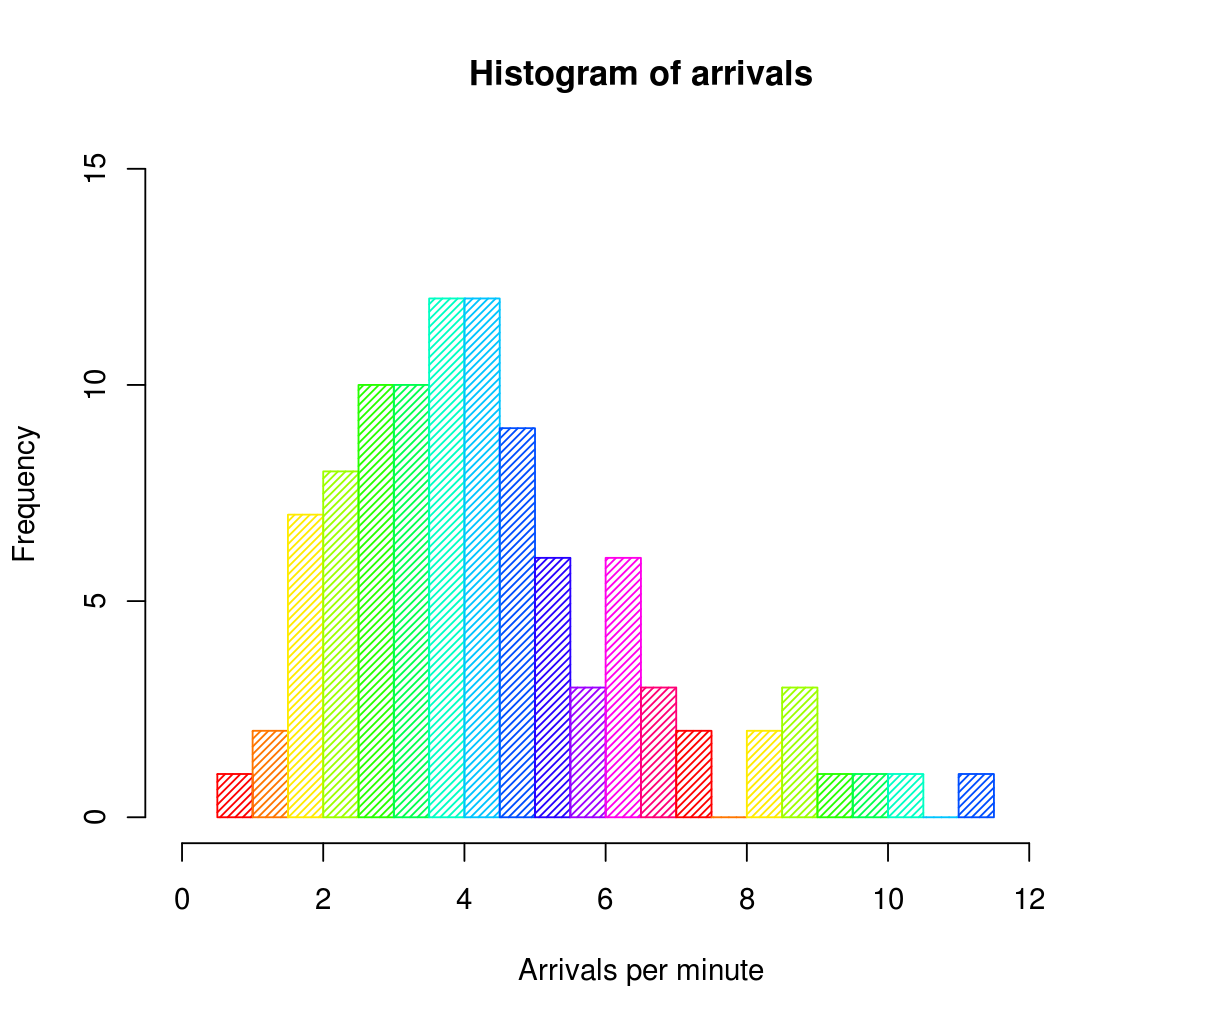
\includegraphics[width=0.95\textwidth,trim={0 1cm 0 5cm},clip]{P02hist.png}
			\credits{By Daniel Penfield at Wikipedia Commons. CC BY-SA 3.0.}
		\end{fig}
\begin{famo}[John Tukey]{famo:tukey}
		\emph{John Wilder Tukey} (June 16, 1915 – July 26, 2000) was an American mathematician.	Born in New Bedford, Massachusetts, he earned a B.A. in 1936 and M.Sc. in 1937, in chemistry, from Brown University, before moving to Princeton University where he received a Ph.D. in mathematics. 
	
	During World War II, he worked at the Fire Control Research Office and collaborated with Samuel Wilks and William Cochran. After the war, he returned to Princeton, where he divided his time between the university and AT\&T Bell Laboratories. \emph{He became a full professor at 35 and was founding chairman of the Princeton statistics department in 1965}. 
	
	He was awarded the \emph{National Medal of Science by President Nixon in 1973}, and the IEEE Medal of Honor in 1982 \enquote{For his contributions to the spectral analysis of random processes and the fast Fourier transform (FFT) algorithm}.

	He is known for developing the FFT algorithm, the box plot, the Tukey range test, the Tukey $\lambda$ distribution, the Tukey test of additivity, and the Teichmüller–Tukey lemma. 
	
	He also made many contributions and articulated the important distinction between exploratory data analysis and confirmatory data analysis. In particular, he believed that much statistical methodology placed too great an emphasis on the latter. A. D. Gordon offered the following summary of Tukey's principles for statistics: 
	\begin{itemize}
		\setlength{\itemsep}{0pt}
		\setlength{\parskip}{0pt} 		
		\item The usefulness and limitation of mathematical statistics, 
		\item \emph{the importance of having methods of statistical analysis that are robust to violations of the assumptions underlying their use},  
		\item the need to amass experience of the behavior of specific methods of analysis in order to provide guidance on their use,  
		\item the importance of \emph{allowing the possibility of data's influencing the choice of method by which they are analyzed}, 
		\item the need for statisticians to reject the role of 'guardian of proven truth', and to resist attempts to provide once-for-all solutions and tidy overunifications, 
		\item the iterative nature of data analysis, and 
		\item the importance of the increasing power, availability and cheapness of computers,
		\item with John von Neumann, he introduced the word \enquote{bit} short for \enquote{binary digit}. 
		\item Tukey's 1958 paper \enquote{The Teaching of Concrete Mathematics} contained the earliest known usage of the term \enquote{software}.
	\end{itemize}
	\credits{Source: \url{https://en.wikipedia.org/wiki/John_Tukey}}
\end{famo}				
	\subsubsection{Box plots}
		Box plots as in figure \ref{fig:boxplot} are another method to display the distribution of a dataset. They can either be shown horizontally or vertically. The box displays the \emph{interquartile range (IQR)} range in which 50\% of the data points are lying. The bar in the box is showing the \nth{2} quartile, the median. The lines extending the box, the so called whiskers or antennas, show the area of 1.5 IQR (in the most cases, but there are also other conventions for the meaning of the whiskers). Outliers are displayed as dots for single values outside of the whiskers.			
		\begin{fig}[Box plot]{fig:boxplot}{!htb}
			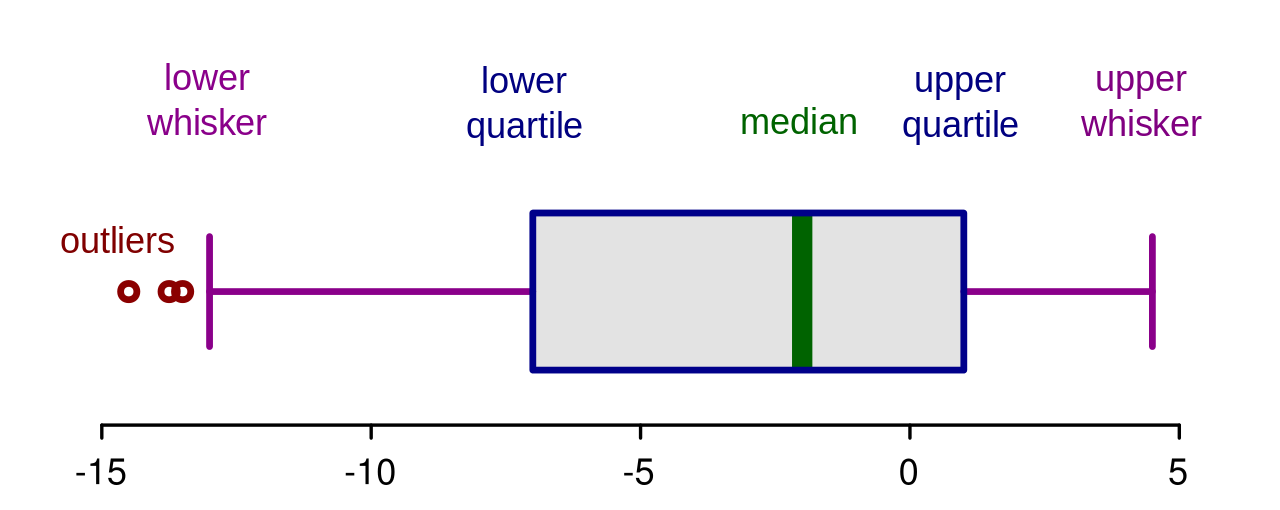
\includegraphics[width=\textwidth,trim={0.5cm .5cm 0.5cm 6cm},clip]{P03box.png}
			\credits{By Ruediger85 at Wikipedia Commons. CC BY-SA 3.0.}
		\end{fig}
	\subsubsection{Pie charts}
		Pie charts are a useful tool to display the shares of different categories. However, they only work out well for relative values and can have a lack of clarity if many small values are included.		
%		\begin{fig}[Pie chart]{fig:pie}{!h}
%			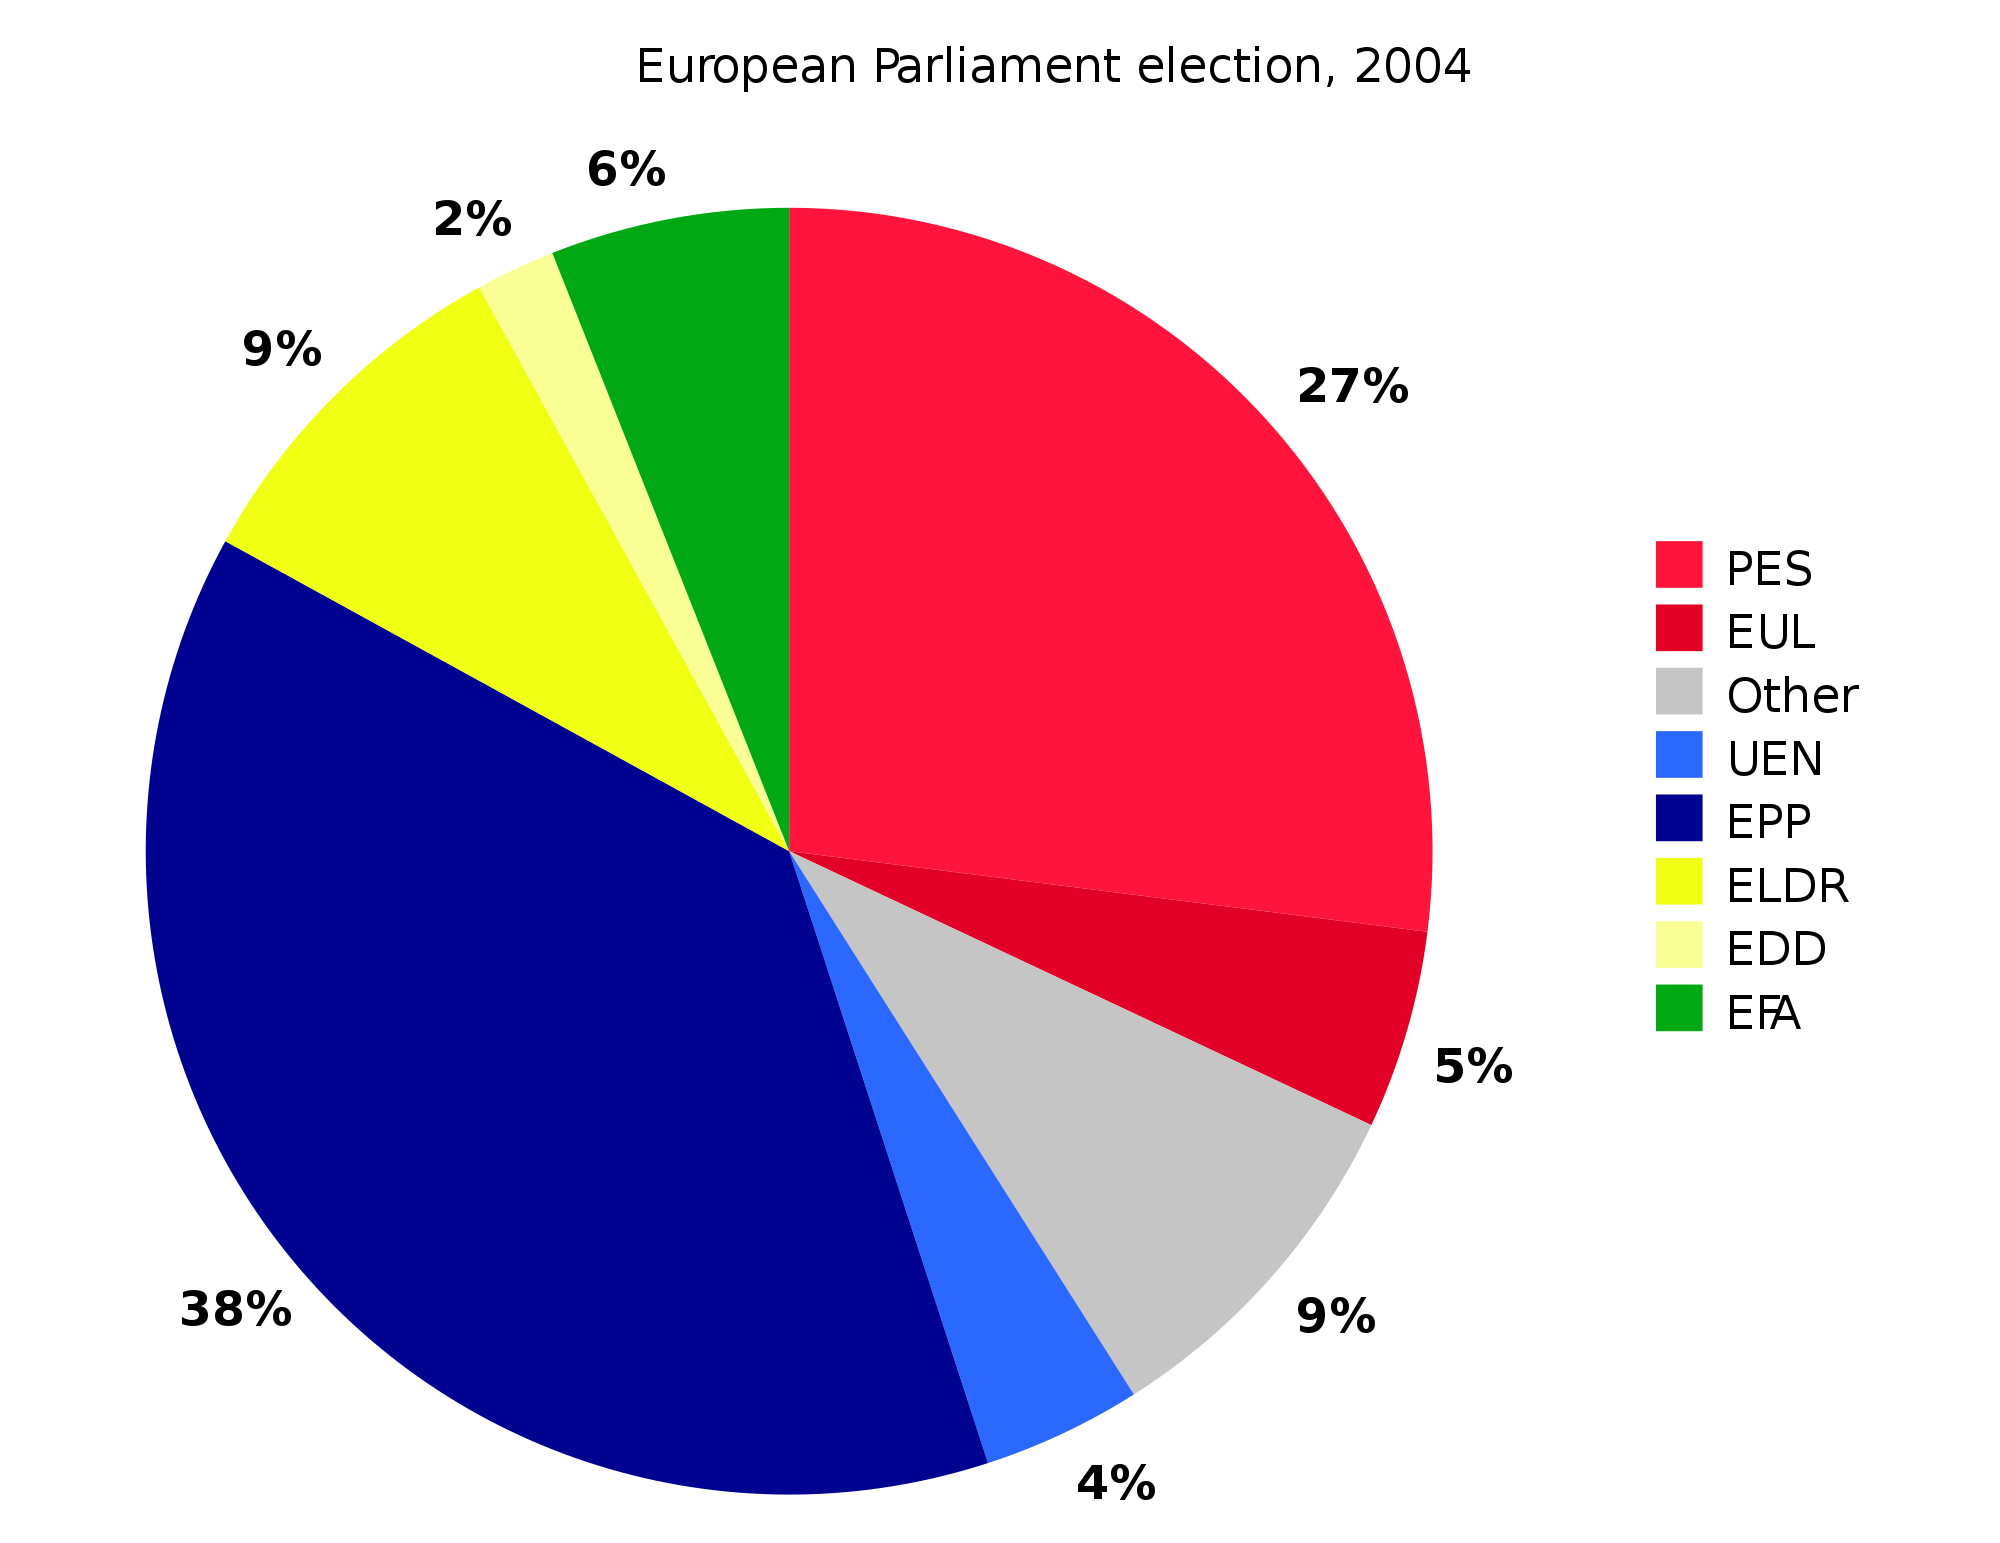
\includegraphics[width=\textwidth,trim={1cm .5cm 3cm 4cm},clip]{P04pie.png}
%			\credits{By Liftarn at Wikipedia Commons. Public Domain.}
%		\end{fig}
	\subsubsection{Scatter plots}
		Scatter plots as in \ref{fig:scatter} display datapoints in a Cartesian coordinate system. This can be done in one to three dimensions, but it is mostly common in two dimensions. Another variable can be displayed by adding color or symbol coding. Scatter plots are helpful to find clusters and get a general idea of how the distribution of the data looks like.				
		\begin{fig}[Scatter plot]{fig:scatter}{!htb}
			\centering{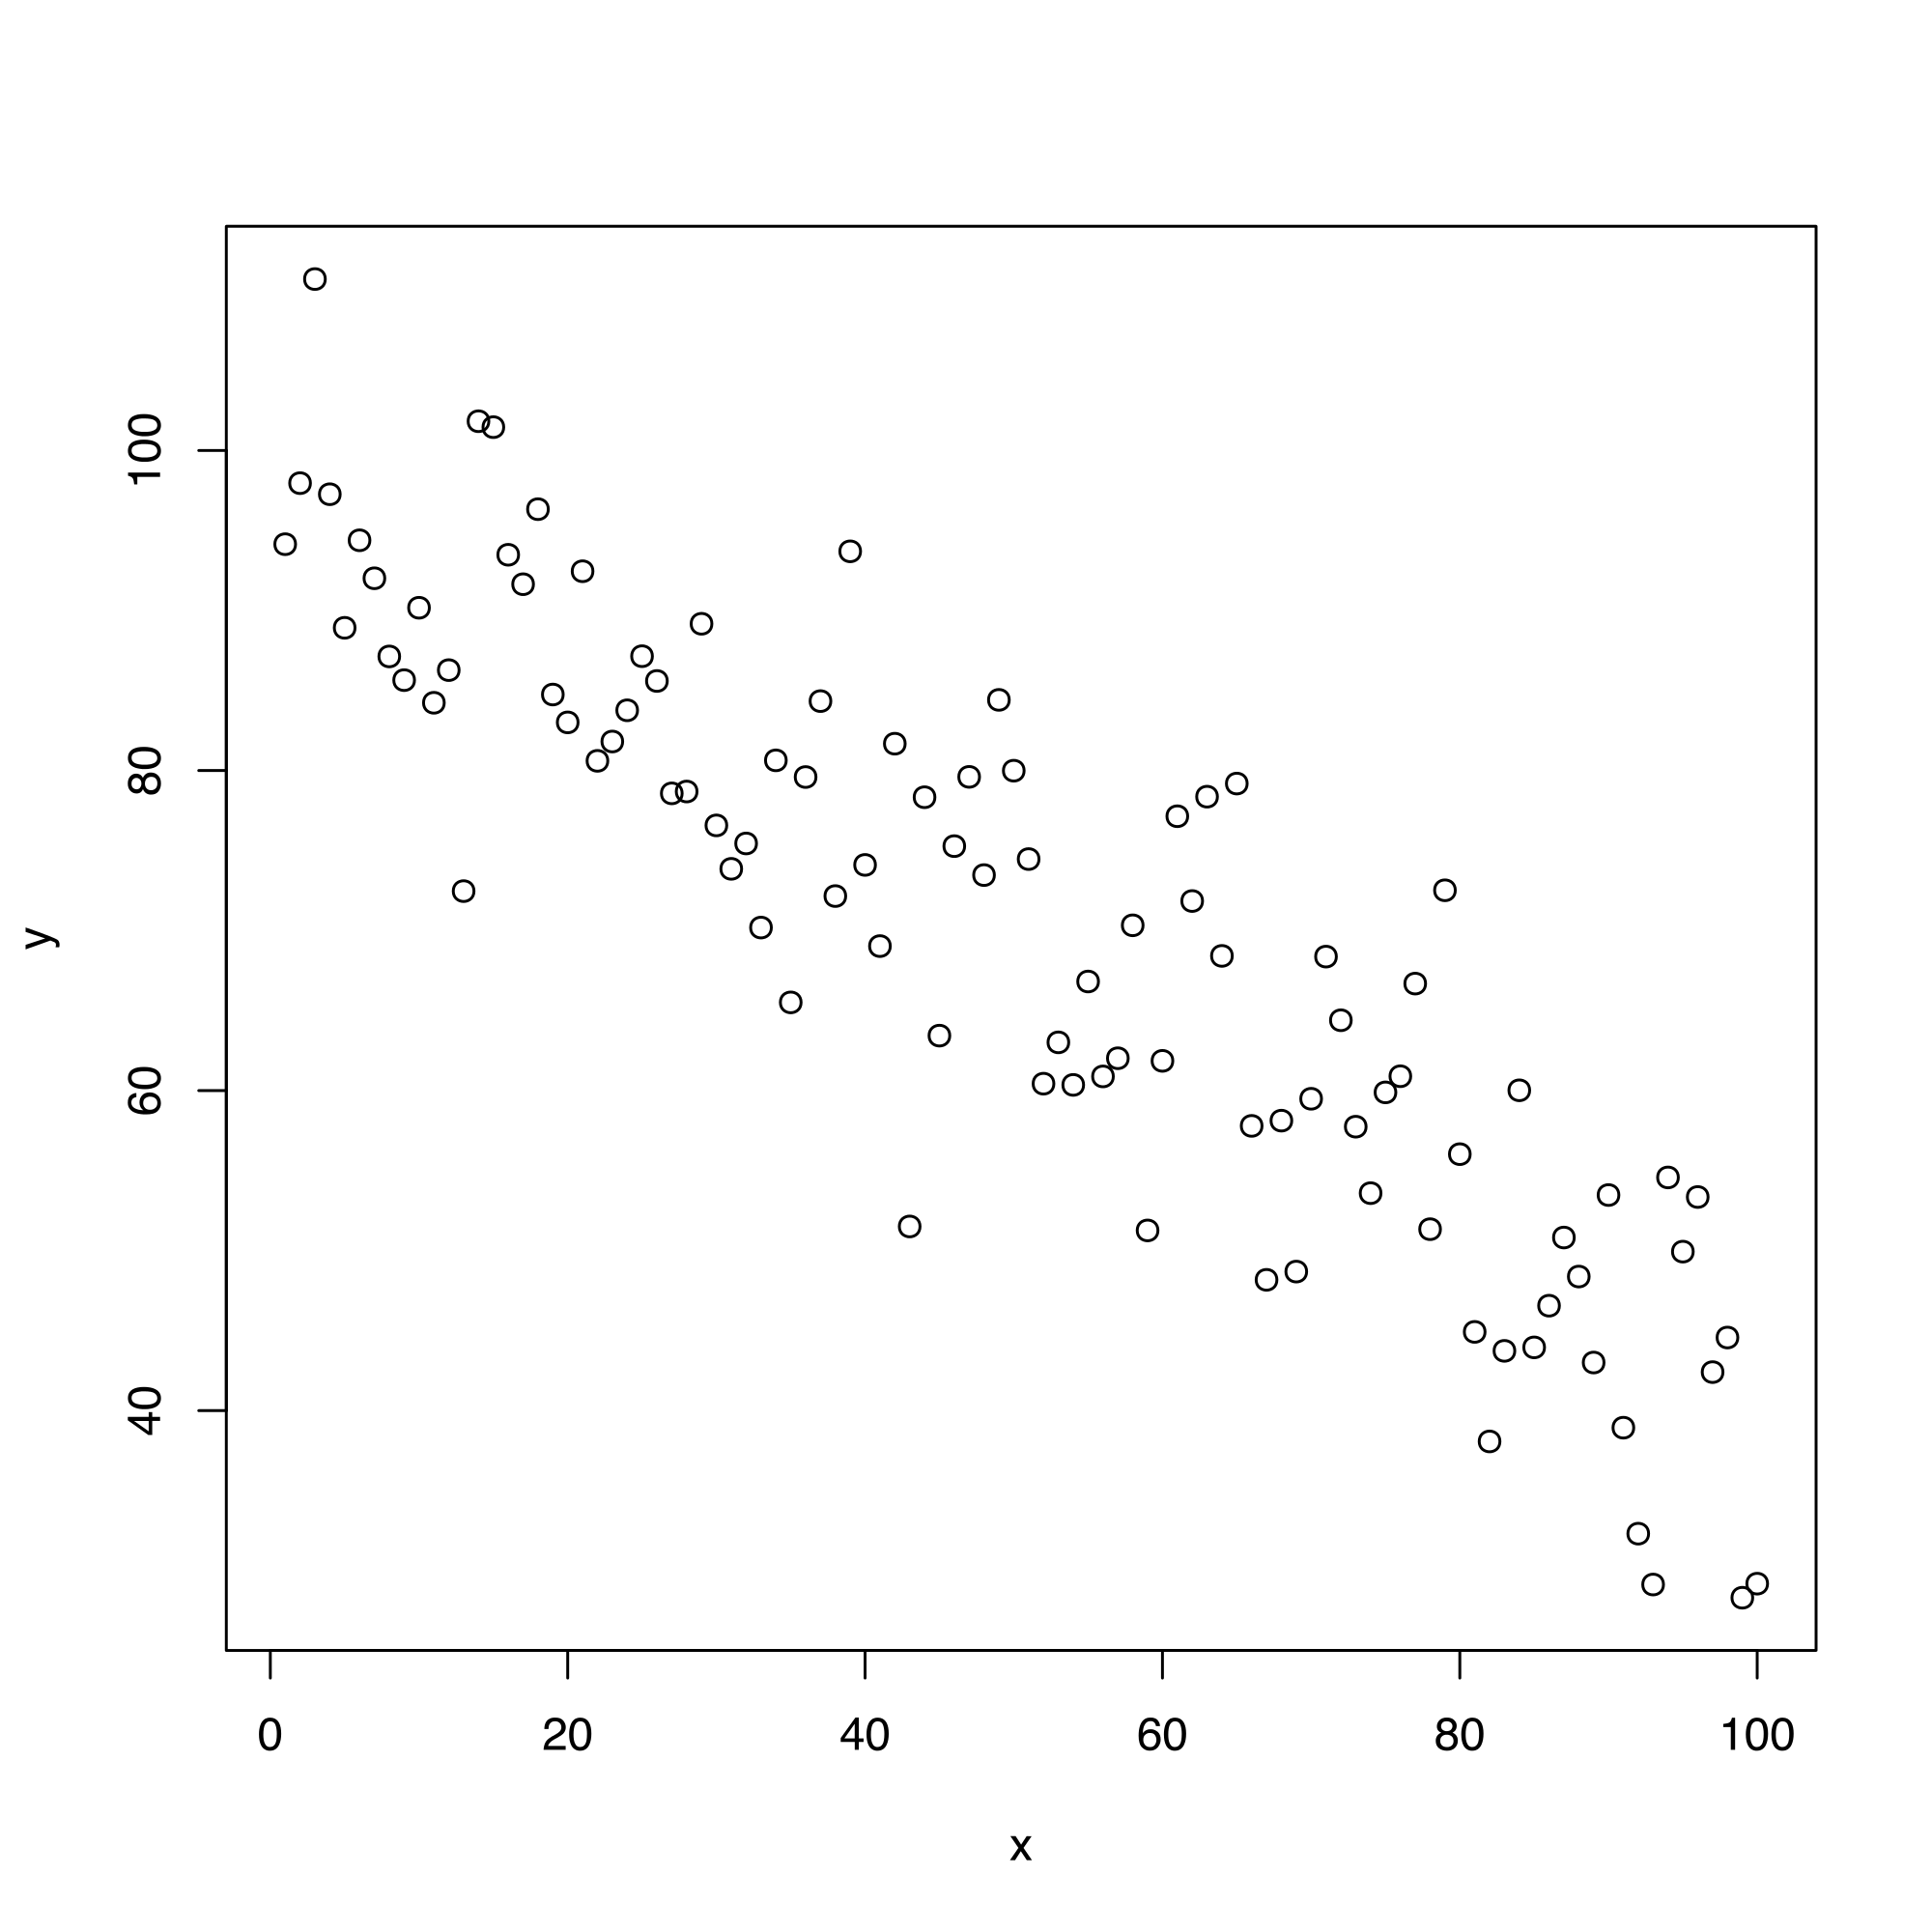
\includegraphics[trim={1cm 2cm 3cm 7cm},clip,width=0.7\textwidth]{P05scatter.png}}
			\credits{By Stiegenaufgang at Wikipedia Commons. CC BY-SA 3.0.}
		\end{fig}				
	\subsubsection{Radar charts}
		Radar charts, also known as spider plots, are shown in figure \ref{fig:radar}. These kind of plots are useful to display how multiple variables changes in different datasets.	This can be helpful to find clusters or outliers in a dataset.								
		\begin{fig}[Spider plot]{fig:radar}{!htb}
			\centering{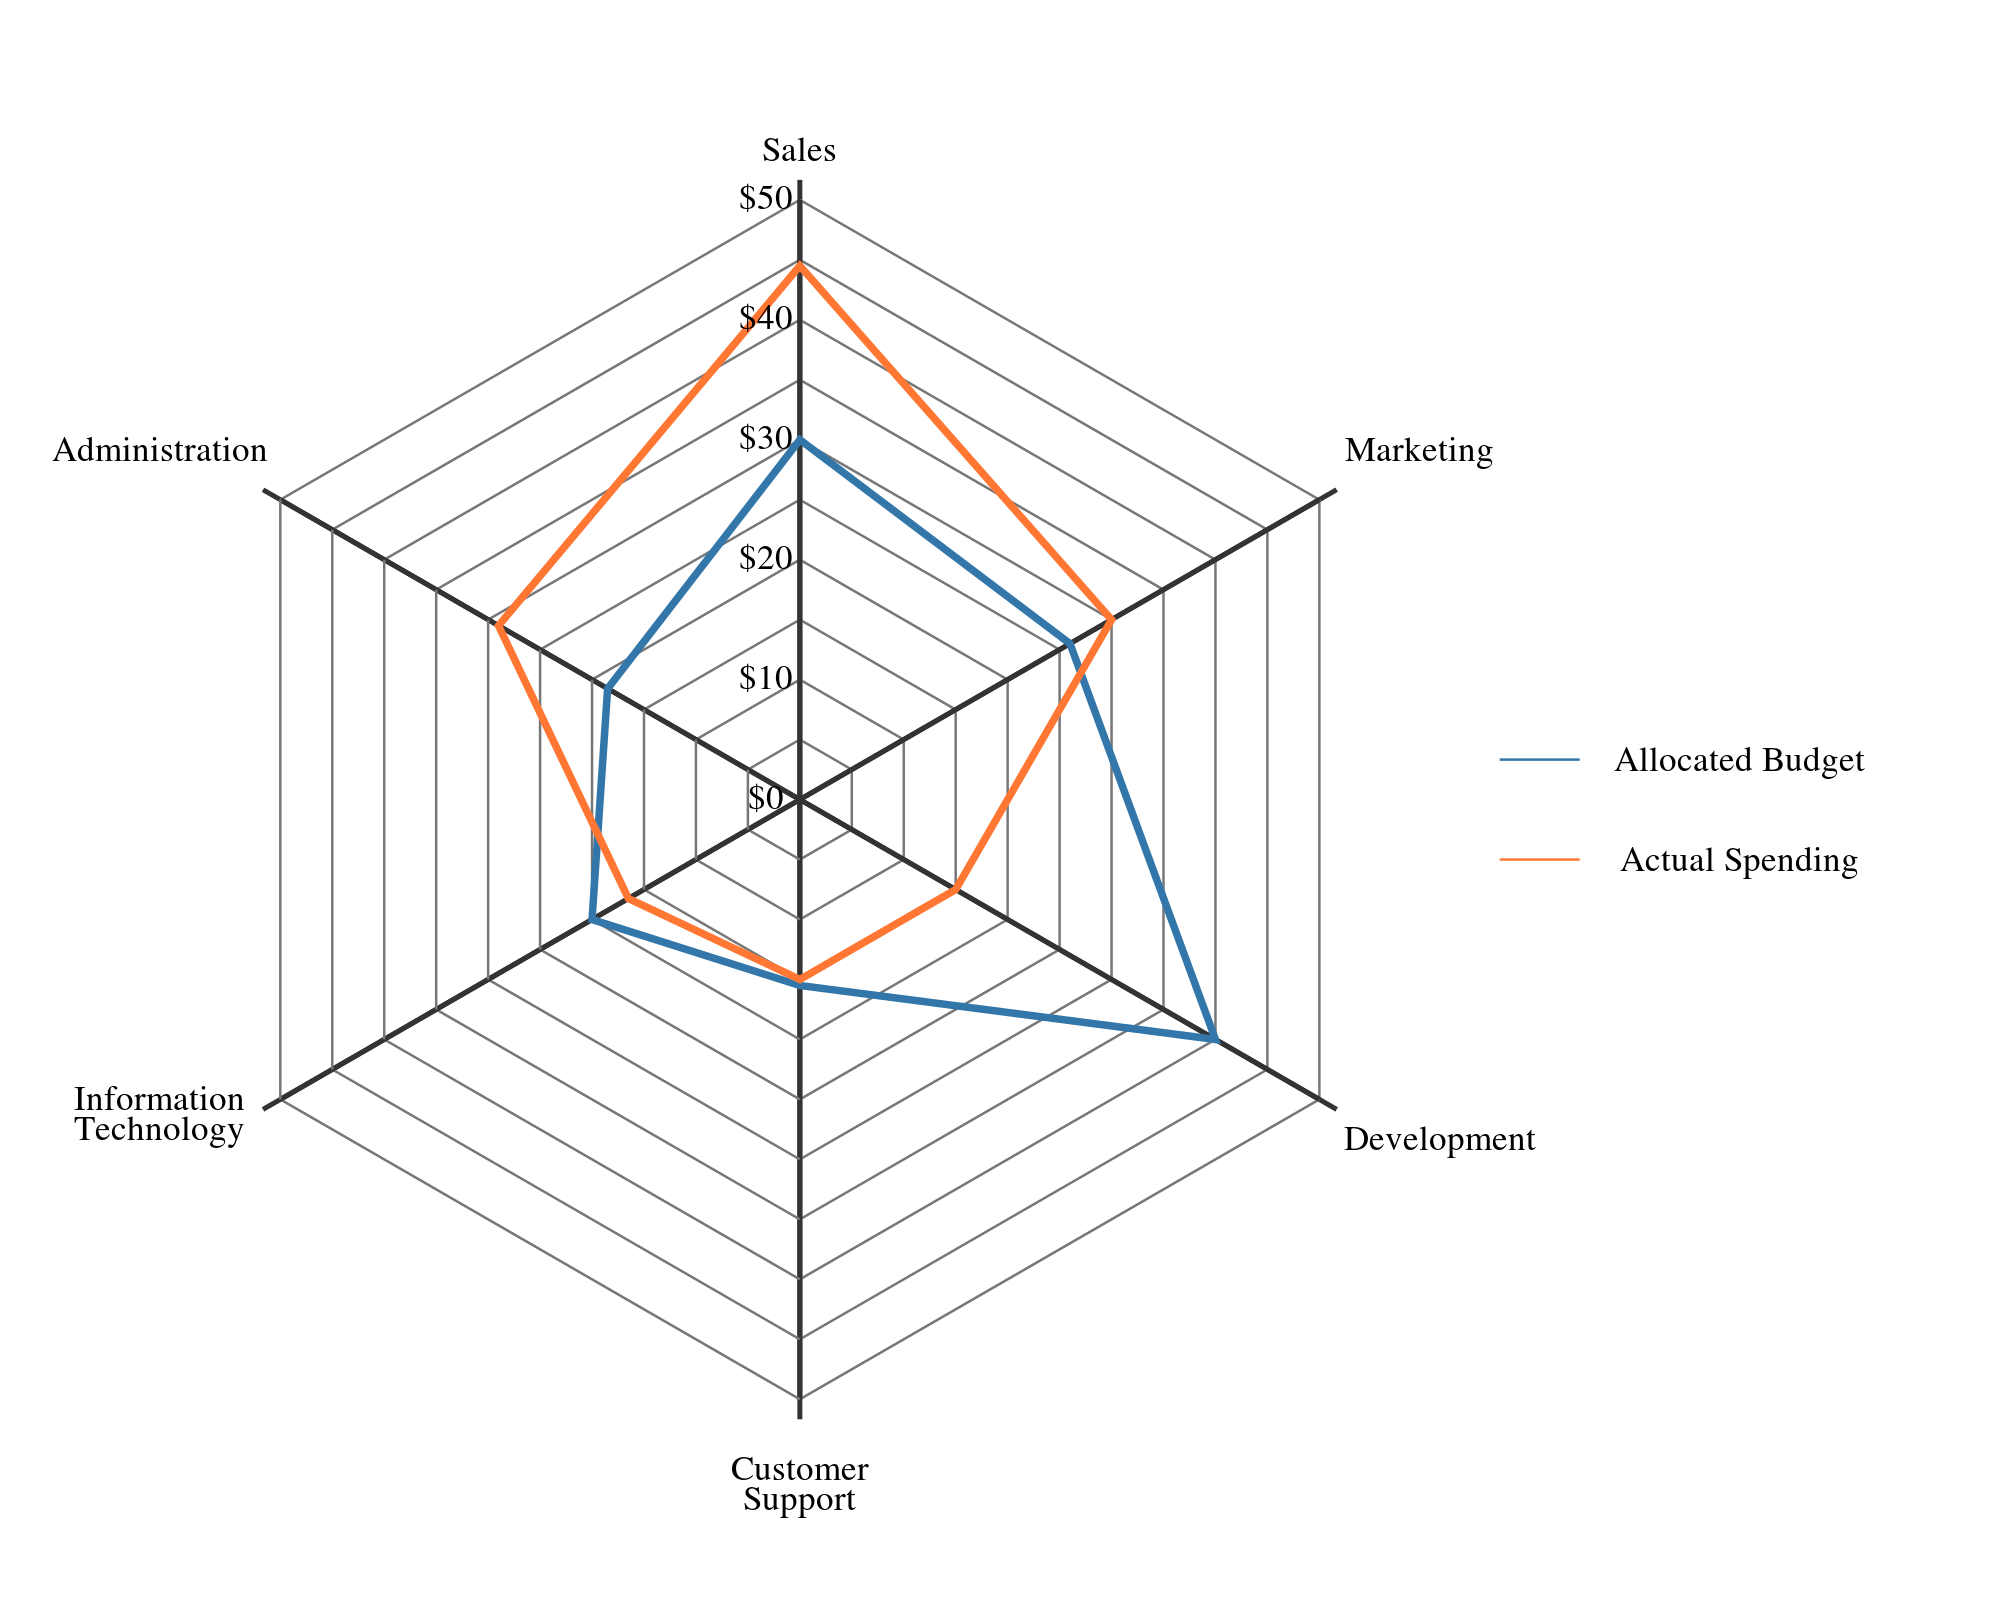
\includegraphics[width=0.7\textwidth,trim={3cm 4.5cm 4.5cm 5.5cm}]{P06radar.png}}
			\credits{Public Domain.}
		\end{fig}		
\subsection{Properties of Estimators}
	Estimators as described in definition \ref{defi:estimator} are important to make statements about the population from a sample. There are many ways to create estimates, and some deliver better results than others.There are some properties that are important for an estimator to be a good estimator.
	\subsubsection{Unbiasedness}
		An estimator is \emph{unbiased} if its expected value is the value of the population parameter of interest $\Theta$. In figure \ref{fig:bias}, the estimator $T_1$ is unbiased because $E(T_1)=\Theta$. The estimator $T_2$ has a bias which is the deviation of its expected value to the population parameter of interest.
		\begin{exmp}[Unbiased Estimator of the population mean]{exmp:bias}
			Consider a random sample
			\begin{equation*}
				\bar{x}=\frac{\sum\limits_{i=1}^n x_i}{n}
			\end{equation*}
			generated by $x_1,x_2,...,x_n$ where the $x_i$ have the same distribution $E(x_i)=\mu$.
			\begin{equation*}
			E\left(\bar{x}\right)=E\left(\frac{\sum\limits_{i=1}^n x_i}{n}\right)=\frac{1}{n} \sum\limits_{i=1}^n E\left(x_i\right)=\frac{1}{n} \sum\limits_{i=1}^n \mu=\frac{n\mu}{n}=\mu
			\end{equation*}
		\end{exmp}
		\begin{fig}[Unbiasedness of an Estimator]{fig:bias}{!htb}
			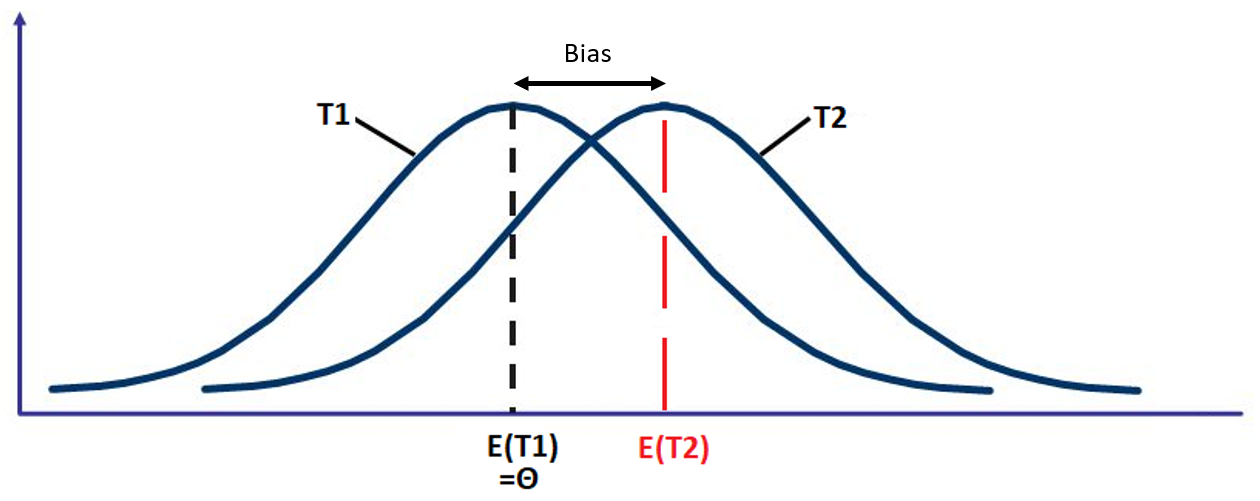
\includegraphics[width=\textwidth]{P07bias.png}
		\end{fig}
	\subsubsection{Efficiency}
		Consider two unbiased estimators $T_1,T_2$ of the same population parameter $\Theta$. $T_1$ is more \emph{efficient} than $T_2$ because if it has a smaller variance as shown in \ref{fig:efficiency}.
		\begin{fig}[Efficiency of an Estimator]{fig:efficiency}{!htb}
			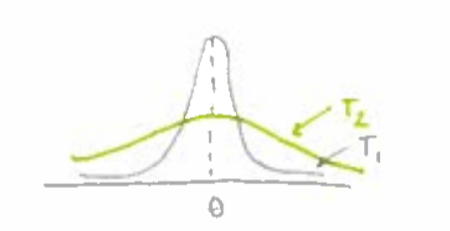
\includegraphics[width=\textwidth,trim={0cm 0cm 0cm .5cm},clip]{P08efficiency.png}
		\end{fig}		
	\subsubsection{Consistency}
		An estimator is \emph{consistent} if the probability that it generates estimates with a small error compared to the population parameter of interest increases to 1 as the sample size becomes infinitely large as shown in figure \ref{fig:consistency}.
		\begin{equation*}
			\forall\,\varepsilon > 0,\qquad \lim\limits_{n\rightarrow+\infty}P_s(|\hat{\Theta}_n-\Theta|>\varepsilon)=0
		\end{equation*}
		with $\hat{\Theta}_n$ as the value of an estimate for $\Theta$ when the sample size is $n$.
	\subsubsection{Sufficiency}
		An estimator is \emph{sufficient} if it contains all information in a sample about the population parameter of interest.
	\subsubsection{Trade-off between unbiasedness and efficiency}
		For an estimator, unbiasedness is desirable but not the only crucial factor. In figure \ref{fig:mse}, we need to decide whether $T_1$ or $T_2$ is the better estimator. This can be determined by calculating the \emph{mean squared error (MSE)}, and the estimator delivering the smallest MSE is the best.
		\begin{equation*}
			MSE(T_1)=var(T)+bias\left(E(T),\Theta\right)
		\end{equation*}
		\begin{fig}[Consistency of an Estimator]{fig:consistency}{!htb}
			\includegraphics[width=\textwidth,trim={0cm 0cm 0.5cm .5cm},clip]{P09Consistency.png}
		\end{fig}			
		\begin{fig}[Mean Square Error an Estimator]{fig:mse}{!htb}
			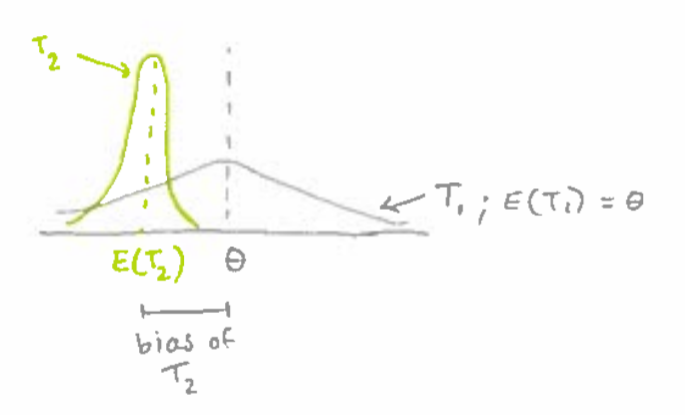
\includegraphics[width=\textwidth]{P10mse.png}
		\end{fig}			
	\subsubsection{Central Limit Theorem (CLT)}\label{sec:clt}
		Consider a sequence of random variables $x_1,x_2,...,x_n$ which are independent identically distributed (i.i.d.) such that $E(x_i)=\mu,\,var(x_i)=\sigma^2$. We are interested in the random variable
		\begin{equation*}
			s_n=\frac{\sum\limits_{i=1}^n x_i}{n}.
		\end{equation*}
		The CLT states that as $n\rightarrow+\infty$ $s_n$ becomes approximately normally distributed with mean $\mu$ and variance $\frac{\sigma^2}{n}$.
		\begin{equation*}
			\sqrt{n}(s_n-\mu)\xrightarrow{d}N(0,\sigma^2),\qquad \xrightarrow{d}\text{ indicates in distribution.}
		\end{equation*}
		Important information we get from this:
		\begin{itemize}
			\item The variance of $s_n$ decreases linearly with $n$, and
			\item $s_n$ is approximately normally distributed with mean $\mu$, so it is \emph{unbiased}.
		\end{itemize}
